\documentclass[tikz,border=7pt]{standalone}
\usepackage[T1]{fontenc}
\usepackage{lmodern}
\usepackage{helvet}
\renewcommand{\familydefault}{\sfdefault}
\usepackage{amsmath}
\usepackage{xcolor}
\usepackage{tikz}
\usetikzlibrary{
  arrows.meta,
  positioning,
  calc,
  fit,
  shapes.geometric,
  shapes.symbols,
  backgrounds,
  decorations.pathreplacing,
  decorations.pathmorphing,
}

\definecolor{slate}{HTML}{334155}
\definecolor{teal}{HTML}{0D9488}
\definecolor{amber}{HTML}{D97706}
\definecolor{rose}{HTML}{E11D48}
\definecolor{muted}{HTML}{64748B}
\definecolor{line}{HTML}{94A3B8}
\definecolor{pagebg}{HTML}{F8FAFC}
\definecolor{card}{HTML}{FFFFFF}
\definecolor{lightteal}{HTML}{CCFBF1}
\definecolor{lightamber}{HTML}{FEF3C7}
\definecolor{lightrose}{HTML}{FFE4E6}
\definecolor{lightslate}{HTML}{E2E8F0}
\definecolor{blueink}{HTML}{2563EB}
\definecolor{bluewash}{HTML}{DBEAFE}
\definecolor{greenink}{HTML}{16A34A}
\definecolor{greenwash}{HTML}{DCFCE7}
\definecolor{pinkink}{HTML}{DB2777}
\definecolor{pinkwash}{HTML}{FCE7F3}

\tikzset{
  >=Stealth,
  font=\sffamily\scriptsize,
  every node/.append style={text=slate},
  title/.style={font=\sffamily\bfseries\small, text=slate, anchor=west},
  note/.style={font=\sffamily\tiny, text=muted, align=left},
  label/.style={font=\sffamily\tiny, text=muted},
  chip/.style={
    draw=#1,
    fill=#1!12,
    rounded corners=2pt,
    inner sep=2.5pt,
    font=\sffamily\tiny\bfseries,
    text=slate,
  },
  decision/.style={
    shape=diamond,
    aspect=2.1,
    draw=teal,
    fill=lightteal,
    inner sep=1.5pt,
    align=center,
    font=\sffamily\tiny,
    text=slate,
  },
  pics/person/.style 2 args={
    code={
      \fill[#1] (0,0.92) circle (0.18);
      \fill[#1]
        (-0.26,0.68)
        .. controls (-0.34,0.42) and (-0.30,0.18) .. (-0.22,0.02)
        -- (0.22,0.02)
        .. controls (0.30,0.18) and (0.34,0.42) .. (0.26,0.68)
        -- cycle;
      \node[font=\sffamily\tiny\bfseries, text=#1, anchor=north] at (0,-0.08) {#2};
    }
  },
  pics/disk/.style={
    code={
      \fill[lightslate] (0,-0.04) ellipse (0.28 and 0.10);
      \fill[slate] (-0.28,-0.04) rectangle (0.28,0.12);
      \fill[slate] (0,0.12) ellipse (0.28 and 0.10);
      \fill[card] (0,0.14) ellipse (0.11 and 0.04);
    }
  },
}

\begin{document}
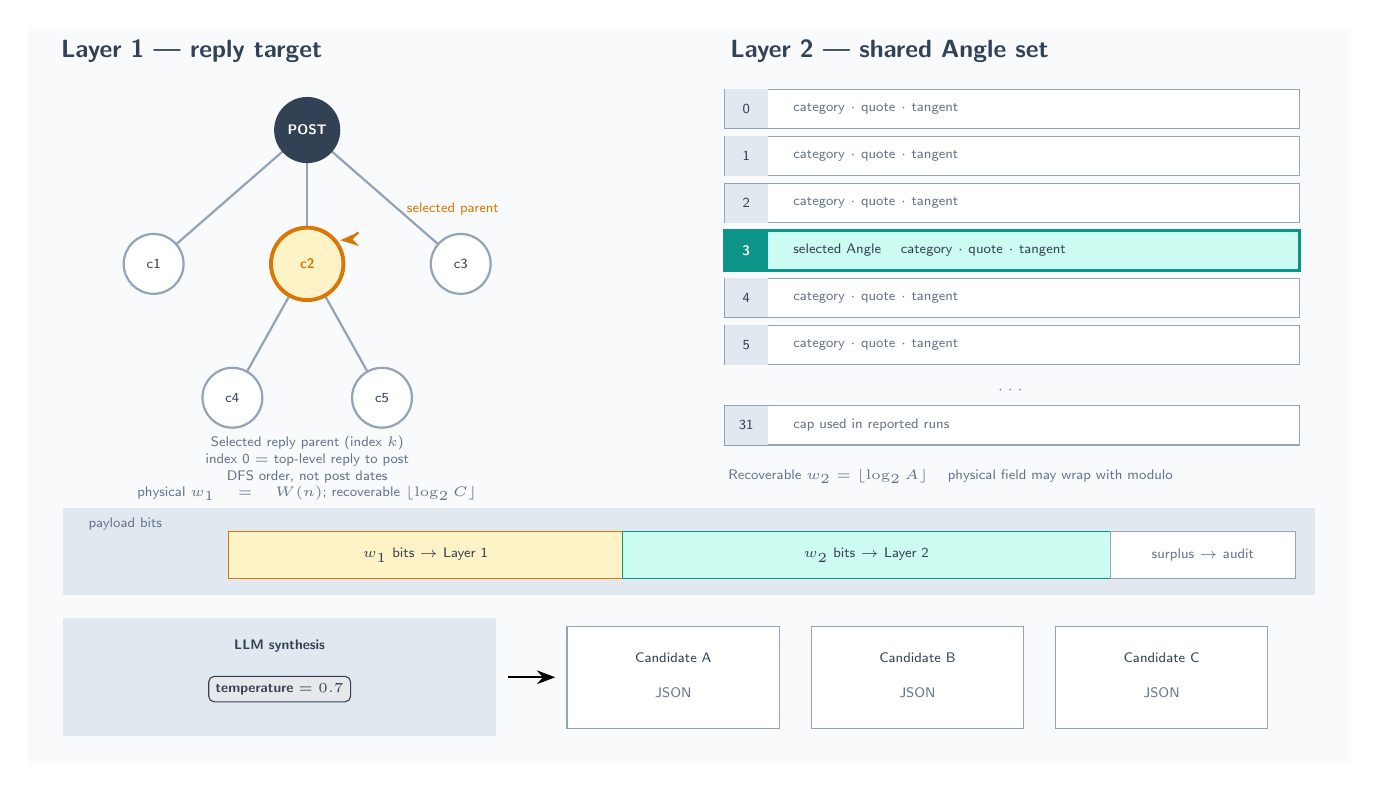
\begin{tikzpicture}[x=1cm,y=1cm]
  \fill[pagebg] (-0.25,-0.2) rectangle (16.55,9.15);
  \node[title] at (0.05,8.85) {Layer 1 --- reply target};
  \node[title] at (8.55,8.85) {Layer 2 --- shared Angle set};

  % --- tree ---
  \coordinate (P) at (3.3,7.85);
  \coordinate (C1) at (1.35,6.15);
  \coordinate (C2) at (3.3,6.15);
  \coordinate (C3) at (5.25,6.15);
  \coordinate (C4) at (2.35,4.45);
  \coordinate (C5) at (4.25,4.45);
  \foreach \a/\b in {P/C1,P/C2,P/C3,C2/C4,C2/C5} {
    \draw[line, thick] (\a) -- (\b);
  }
  \fill[slate] (P) circle (0.42);
  \node[font=\sffamily\tiny\bfseries, text=card] at (P) {POST};
  \foreach \c/\lab in {C1/c1, C3/c3, C4/c4, C5/c5} {
    \fill[card] (\c) circle (0.38);
    \draw[line, thick] (\c) circle (0.38);
    \node[font=\sffamily\tiny] at (\c) {\lab};
  }
  \fill[lightamber] (C2) circle (0.46);
  \draw[amber, line width=1.4pt] (C2) circle (0.46);
  \node[font=\sffamily\tiny\bfseries, text=amber] at (C2) {c2};
  \draw[amber, thick, ->] (3.95,6.55) to[bend left=20] (3.72,6.45);
  \node[font=\sffamily\tiny, text=amber] at (5.15,6.85) {selected parent};

  \node[note, align=center, text width=6.6cm] at (3.3,3.55) {%
    Selected reply parent (index $k$)\\
    index 0 $=$ top-level reply to post\\
    DFS order, not post dates\\
    physical $w_1=W(n)$; recoverable $\lfloor\log_2 C\rfloor$};

  % --- angle tickets ---
  \foreach \i/\y/\sel in {
    0/8.15/0, 1/7.55/0, 2/6.95/0, 3/6.35/1,
    4/5.75/0, 5/5.15/0} {
    \ifnum\sel=1
      \fill[lightteal] (8.6,\y-0.28) rectangle (15.9,\y+0.22);
      \draw[teal, line width=1.2pt] (8.6,\y-0.28) rectangle (15.9,\y+0.22);
      \fill[teal] (8.6,\y-0.28) rectangle (9.15,\y+0.22);
      \node[font=\sffamily\tiny\bfseries, text=card] at (8.875,\y-0.03) {\i};
      \node[font=\sffamily\tiny, anchor=west] at (9.35,\y-0.03) {selected Angle \quad category $\cdot$ quote $\cdot$ tangent};
    \else
      \fill[card] (8.6,\y-0.28) rectangle (15.9,\y+0.22);
      \draw[line] (8.6,\y-0.28) rectangle (15.9,\y+0.22);
      \fill[lightslate] (8.6,\y-0.28) rectangle (9.15,\y+0.22);
      \node[font=\sffamily\tiny] at (8.875,\y-0.03) {\i};
      \node[font=\sffamily\tiny, text=muted, anchor=west] at (9.35,\y-0.03) {category $\cdot$ quote $\cdot$ tangent};
    \fi
  }
  \node[font=\sffamily\tiny, text=muted] at (12.25,4.55) {$\cdots$};
  \fill[card] (8.6,3.85) rectangle (15.9,4.35);
  \draw[line] (8.6,3.85) rectangle (15.9,4.35);
  \fill[lightslate] (8.6,3.85) rectangle (9.15,4.35);
  \node[font=\sffamily\tiny] at (8.875,4.10) {31};
  \node[font=\sffamily\tiny, text=muted, anchor=west] at (9.35,4.10) {cap used in reported runs};

  \node[note, text width=7.2cm] at (12.25,3.45) {Recoverable $w_2=\lfloor\log_2 A\rfloor$ \quad physical field may wrap with modulo};

  % bitstream
  \fill[lightslate] (0.2,1.95) rectangle (16.1,3.05);
  \node[label, anchor=west] at (0.4,2.85) {payload bits};
  \fill[lightamber] (2.3,2.15) rectangle (7.3,2.75);
  \draw[amber] (2.3,2.15) rectangle (7.3,2.75);
  \node[font=\sffamily\tiny] at (4.8,2.45) {$w_1$ bits $\rightarrow$ Layer 1};
  \fill[lightteal] (7.3,2.15) rectangle (13.5,2.75);
  \draw[teal] (7.3,2.15) rectangle (13.5,2.75);
  \node[font=\sffamily\tiny] at (10.4,2.45) {$w_2$ bits $\rightarrow$ Layer 2};
  \fill[card] (13.5,2.15) rectangle (15.85,2.75);
  \draw[line] (13.5,2.15) rectangle (15.85,2.75);
  \node[label] at (14.675,2.45) {surplus $\rightarrow$ audit};

  % synthesis
  \fill[lightslate] (0.2,0.15) rectangle (5.7,1.65);
  \node[font=\sffamily\tiny\bfseries] at (2.95,1.30) {LLM synthesis};
  \node[chip=slate] at (2.95,0.75) {temperature $=0.7$};
  \draw[thick, ->] (5.85,0.90) -- (6.45,0.90);
  \foreach \x/\lab in {6.6/A, 9.7/B, 12.8/C} {
    \fill[card] (\x,0.25) rectangle (\x+2.7,1.55);
    \draw[line] (\x,0.25) rectangle (\x+2.7,1.55);
    \node[font=\sffamily\tiny] at (\x+1.35,1.15) {Candidate \lab};
    \node[label] at (\x+1.35,0.70) {JSON};
  }
\end{tikzpicture}
\end{document}
